\documentclass[sigplan,screen]{acmart}
\def\BibTeX{{\rm B\kern-.05em{\sc i\kern-.025em b}\kern-.08emT\kern-.1667em\lower.7ex\hbox{E}\kern-.125emX}}

\copyrightyear{2018}
\acmYear{2018}
\setcopyright{acmlicensed}
\acmConference[SER 574]{SER 574}{January 20, 2019}{Mesa, AZ}
\acmBooktitle{SER 574: Assignment 1, January 20, 20198, Mesa, AZ}
\acmPrice{}
\acmDOI{}
\acmISBN{}

\usepackage{times}
\usepackage{graphicx}
\usepackage{url,hyperref}


\begin{document}

\title{Adapting Agile for Large Scale Projects}

\author{Joshua Drumm}
\email{jkdrumm@asu.edu}
\affiliation{%
	\institution{Arizona State University}
}

\author{Jainish Soni}
\email{jjsoni@asu.edu}
\affiliation{%
	\institution{Arizona State University}
}

\date{\today}

\begin{abstract}
Working with multiple agile teams presents new problems compared to working with a single agile team. First explored are some common reasons why it is difficult to work with multiple agile teams. To overcome these new problems, new techniques and positions can be used. While additional communication is important, so is a new structure. Having the software architecture and design well known throughout all teams is vital for success.
\end{abstract}

\keywords{Agile, Scrum, Architecture Owner}

\maketitle

\newpage
\pagenumbering{arabic}


\keywords{Communication, Collaboration, Agile, Organization}

\section{Introduction}
As projects become larger and larger, there becomes a need for more people to complete them. However, scaling agile is not very straight forward. With enough people on one project, there can be many different agile teams all working together. In order to effectively deliver a successful product, there are some additional agile techniques that should be employed by anyone using multiple agile teams.

\section{Questions}

\subsection{What is important for multiple agile teams work together collaboratively?}
In this digital era, for any company to offer better products to the market and complete larger projects on time; the agile method is the key. Agile method is a way of practising Scrum in a company, where self-motivated, specialized and highly effective people work together in a team to get the best results. Although, in a big company, there is a need for multiple agile teams to work together as a team. Ideally, such a scenario should offer better results for the company and different team members should be able to deliver more output. But, in the real world, such a thing does not happen. There are various reasons for the idea to fail in a real-world scenario:
\begin{enumerate}
\item Geographical Limitations \cite{Cross18} - As agile requires to stand up meetings on a daily basis to check the progress made by individuals in the project, team members can be at various geographical locations and would not be able to attend such meetings.
\item Overdependence on some members \cite{Cross18} - There can be a case where a group of members are delivering more than other members. Such a thing can impact the overall nature of the project and can make other members impotent to work.
\item Failure in managing the skills of individual member \cite{Cross18} - Every individual in the team may be consisting of various skills. While working in a number of teams, if any of the members are not assigned the task according to the skill set, then the potential member would not be able to deliver the result.
\end{enumerate}
In order to avoid such issues in agility, it is important that the senior management pay attention to various points to make the agile practice is conducted in a right manner to fulfill the end goals of the project.

\begin{itemize}
\item The objective of the project should be well defined so that every team can have the exact idea of the workflow \cite{SAFe18}.
\item Communication is the biggest concern in agility and it should be removed by creating a more collaborative environment, where team members can share their knowledge and help each other to achieve goals \cite{Agile}.
\item Scrum master should understand the ability and skills of each and every member of the team to assign tasks accordingly which can produce higher output.
\item A new member of the team should be given a chance to get on board and should be paired with an experienced person. Such practice can get the new member acquainted with the process and the environment of the organization.
\item Each team should be given separate work so that redundancy can be avoided and better results can be produced in a very small amount of time \cite{GSA}.
\item Rewarding team members based on their collaboration and their input in the project can bring out the members from isolation and can motivate them to work as a team. This can enhance the performance of the team members which ultimately helps the organization. 
\item Workload should be equally distributed among the members so that over-dependence on some people can be avoided and everyone can feel a part of the team and a sense of accomplishment without being overburdened.
\end{itemize}
So, this is how multiple agile teams should work in an organization to deliver the product in a given time schedule by creating harmony among team members and a sense of contribution to the team. \\


\subsection{Why is Design and Architecture so important when working with multiple agile teams?}
While having a plan to follow is already important enough in software engineering, it is even more important when working with multiple agile teams. In order for teams to stay focused on the goal, the architecture and design must be fully understood across all teams.
In order to achieve this with large or multiple teams, it is important to have an architecture owner in order to avoid conflicts between developers and between teams. This can be an additional role in scrum much like the product owner and the scrum master. While the architecture owner has the ultimate power to influence the direction of the architecture, they should still work with the developers in order to create an architectural environment that the developers can work in easily \cite{WAmbler}. This role is important because without an architecture owner, many developers can disagree on the design of a project. Having an architecture owner can help bring people to agreement, always having the final decision. \par
When dealing with especially large agile teams, it can be beneficial to have a separate team of architecture owners. There would be an architecture owner for each other team, and there would also be a chief architecture owner to oversee the other architecture owners \cite{WAmbler}. The structure for this style of system is visualized in Figure \ref{fig:label1} When using a system like this, there are four approaches to creating the teams: architecture-driven, feature-driven, open source, and combinational \cite{WAmbler}.
The architectural approach involves dividing teams based on the architecture of the system, each team working with a separate component. The feature driven approach divides into teams based on feature implementation. The open source approach is best when many different systems or subsystems are dependent on one another, and allows for each system to be created in an open source manner. The last approach, combinational, is simply a mix of any of the previous approaches. \par
In order to follow an architectural plan with many agile teams, it is important to have a good model of the architecture. The models do not need to be very detailed, but must be understood by every team.

\begin{figure}[!htb]
        \center{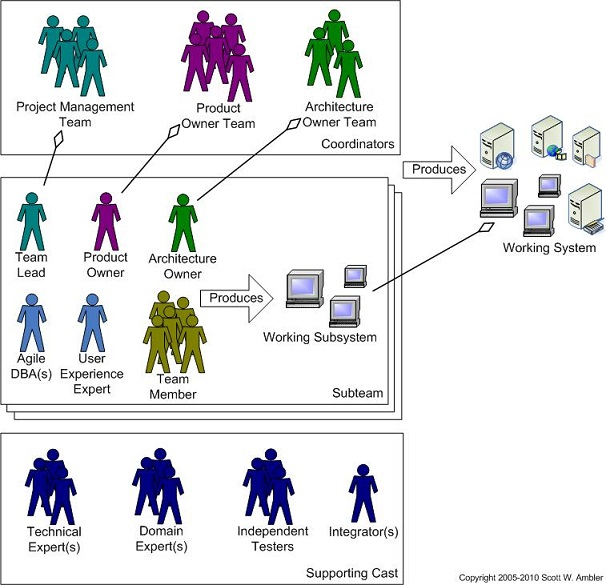
\includegraphics[scale=0.5]{agileTeamLarge.jpg}}
        \caption{\label{fig:label1} How to divide and structure architecture owners among teams \cite{WAmbler}}
\end{figure}

\section{Conclusion}
While the complexity increases greatly when scaling agile, there are techniques to keep it under control. Good communication, supporting scrum masters, resourceful division of labor, and architecture owners can all greatly reduce complexity as well as increase productivity.

\bibliographystyle{ACM-Reference-Format}
\bibliography{Assignment1References}

\end{document}